\documentclass[1p]{elsarticle_modified}
%\bibliographystyle{elsarticle-num}

%\usepackage[colorlinks]{hyperref}
%\usepackage{abbrmath_seonhwa} %\Abb, \Ascr, \Acal ,\Abf, \Afrak
\usepackage{amsfonts}
\usepackage{amssymb}
\usepackage{amsmath}
\usepackage{amsthm}
\usepackage{scalefnt}
\usepackage{amsbsy}
\usepackage{kotex}
\usepackage{caption}
\usepackage{subfig}
\usepackage{color}
\usepackage{graphicx}
\usepackage{xcolor} %% white, black, red, green, blue, cyan, magenta, yellow
\usepackage{float}
\usepackage{setspace}
\usepackage{hyperref}

\usepackage{tikz}
\usetikzlibrary{arrows}

\usepackage{multirow}
\usepackage{array} % fixed length table
\usepackage{hhline}

%%%%%%%%%%%%%%%%%%%%%
\makeatletter
\renewcommand*\env@matrix[1][\arraystretch]{%
	\edef\arraystretch{#1}%
	\hskip -\arraycolsep
	\let\@ifnextchar\new@ifnextchar
	\array{*\c@MaxMatrixCols c}}
\makeatother %https://tex.stackexchange.com/questions/14071/how-can-i-increase-the-line-spacing-in-a-matrix
%%%%%%%%%%%%%%%

\usepackage[normalem]{ulem}

\newcommand{\msout}[1]{\ifmmode\text{\sout{\ensuremath{#1}}}\else\sout{#1}\fi}
%SOURCE: \msout is \stkout macro in https://tex.stackexchange.com/questions/20609/strikeout-in-math-mode

\newcommand{\cancel}[1]{
	\ifmmode
	{\color{red}\msout{#1}}
	\else
	{\color{red}\sout{#1}}
	\fi
}

\newcommand{\add}[1]{
	{\color{blue}\uwave{#1}}
}

\newcommand{\replace}[2]{
	\ifmmode
	{\color{red}\msout{#1}}{\color{blue}\uwave{#2}}
	\else
	{\color{red}\sout{#1}}{\color{blue}\uwave{#2}}
	\fi
}

\newcommand{\Sol}{\mathcal{S}} %segment
\newcommand{\D}{D} %diagram
\newcommand{\A}{\mathcal{A}} %arc


%%%%%%%%%%%%%%%%%%%%%%%%%%%%%5 test

\def\sl{\operatorname{\textup{SL}}(2,\Cbb)}
\def\psl{\operatorname{\textup{PSL}}(2,\Cbb)}
\def\quan{\mkern 1mu \triangleright \mkern 1mu}

\theoremstyle{definition}
\newtheorem{thm}{Theorem}[section]
\newtheorem{prop}[thm]{Proposition}
\newtheorem{lem}[thm]{Lemma}
\newtheorem{ques}[thm]{Question}
\newtheorem{cor}[thm]{Corollary}
\newtheorem{defn}[thm]{Definition}
\newtheorem{exam}[thm]{Example}
\newtheorem{rmk}[thm]{Remark}
\newtheorem{alg}[thm]{Algorithm}

\newcommand{\I}{\sqrt{-1}}
\begin{document}

%\begin{frontmatter}
%
%\title{Boundary parabolic representations of knots up to 8 crossings}
%
%%% Group authors per affiliation:
%\author{Yunhi Cho} 
%\address{Department of Mathematics, University of Seoul, Seoul, Korea}
%\ead{yhcho@uos.ac.kr}
%
%
%\author{Seonhwa Kim} %\fnref{s_kim}}
%\address{Center for Geometry and Physics, Institute for Basic Science, Pohang, 37673, Korea}
%\ead{ryeona17@ibs.re.kr}
%
%\author{Hyuk Kim}
%\address{Department of Mathematical Sciences, Seoul National University, Seoul 08826, Korea}
%\ead{hyukkim@snu.ac.kr}
%
%\author{Seokbeom Yoon}
%\address{Department of Mathematical Sciences, Seoul National University, Seoul, 08826,  Korea}
%\ead{sbyoon15@snu.ac.kr}
%
%\begin{abstract}
%We find all boundary parabolic representation of knots up to 8 crossings.
%
%\end{abstract}
%\begin{keyword}
%    \MSC[2010] 57M25 
%\end{keyword}
%
%\end{frontmatter}

%\linenumbers
%\tableofcontents
%
\newcommand\colored[1]{\textcolor{white}{\rule[-0.35ex]{0.8em}{1.4ex}}\kern-0.8em\color{red} #1}%
%\newcommand\colored[1]{\textcolor{white}{ #1}\kern-2.17ex	\textcolor{white}{ #1}\kern-1.81ex	\textcolor{white}{ #1}\kern-2.15ex\color{red}#1	}

{\Large $\underline{12n_{0460}~(K12n_{0460})}$}

\setlength{\tabcolsep}{10pt}
\renewcommand{\arraystretch}{1.6}
\vspace{1cm}\begin{tabular}{m{100pt}>{\centering\arraybackslash}m{274pt}}
\multirow{5}{120pt}{
	\centering
	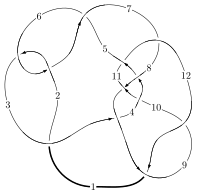
\includegraphics[width=112pt]{../../../GIT/diagram.site/Diagrams/png/2549_12n_0460.png}\\
\ \ \ A knot diagram\footnotemark}&
\allowdisplaybreaks
\textbf{Linearized knot diagam} \\
\cline{2-2}
 &
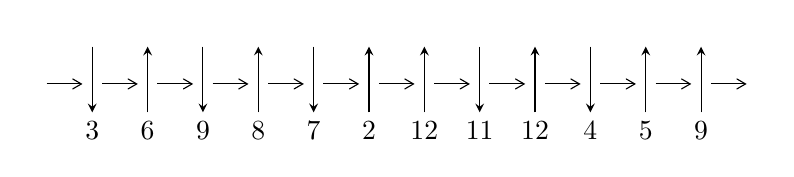
\begin{tikzpicture}[x=20pt, y=17pt]
	% nodes
	\node (C0) at (0, 0) {};
	\node (C1) at (1, 0) {};
	\node (C1U) at (1, +1) {};
	\node (C1D) at (1, -1) {3};

	\node (C2) at (2, 0) {};
	\node (C2U) at (2, +1) {};
	\node (C2D) at (2, -1) {6};

	\node (C3) at (3, 0) {};
	\node (C3U) at (3, +1) {};
	\node (C3D) at (3, -1) {9};

	\node (C4) at (4, 0) {};
	\node (C4U) at (4, +1) {};
	\node (C4D) at (4, -1) {8};

	\node (C5) at (5, 0) {};
	\node (C5U) at (5, +1) {};
	\node (C5D) at (5, -1) {7};

	\node (C6) at (6, 0) {};
	\node (C6U) at (6, +1) {};
	\node (C6D) at (6, -1) {2};

	\node (C7) at (7, 0) {};
	\node (C7U) at (7, +1) {};
	\node (C7D) at (7, -1) {12};

	\node (C8) at (8, 0) {};
	\node (C8U) at (8, +1) {};
	\node (C8D) at (8, -1) {11};

	\node (C9) at (9, 0) {};
	\node (C9U) at (9, +1) {};
	\node (C9D) at (9, -1) {12};

	\node (C10) at (10, 0) {};
	\node (C10U) at (10, +1) {};
	\node (C10D) at (10, -1) {4};

	\node (C11) at (11, 0) {};
	\node (C11U) at (11, +1) {};
	\node (C11D) at (11, -1) {5};

	\node (C12) at (12, 0) {};
	\node (C12U) at (12, +1) {};
	\node (C12D) at (12, -1) {9};
	\node (C13) at (13, 0) {};

	% arrows
	\draw[->,>={angle 60}]
	(C0) edge (C1) (C1) edge (C2) (C2) edge (C3) (C3) edge (C4) (C4) edge (C5) (C5) edge (C6) (C6) edge (C7) (C7) edge (C8) (C8) edge (C9) (C9) edge (C10) (C10) edge (C11) (C11) edge (C12) (C12) edge (C13) ;	\draw[->,>=stealth]
	(C1U) edge (C1D) (C2D) edge (C2U) (C3U) edge (C3D) (C4D) edge (C4U) (C5U) edge (C5D) (C6D) edge (C6U) (C7D) edge (C7U) (C8U) edge (C8D) (C9D) edge (C9U) (C10U) edge (C10D) (C11D) edge (C11U) (C12D) edge (C12U) ;
	\end{tikzpicture} \\
\hhline{~~} \\& 
\textbf{Solving Sequence} \\ \cline{2-2} 
 &
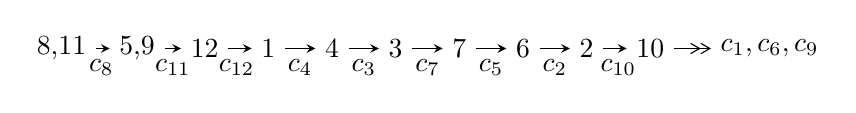
\begin{tikzpicture}[x=23pt, y=7pt]
	% node
	\node (A0) at (-1/8, 0) {8,11};
	\node (A1) at (17/16, 0) {5,9};
	\node (A2) at (17/8, 0) {12};
	\node (A3) at (25/8, 0) {1};
	\node (A4) at (33/8, 0) {4};
	\node (A5) at (41/8, 0) {3};
	\node (A6) at (49/8, 0) {7};
	\node (A7) at (57/8, 0) {6};
	\node (A8) at (65/8, 0) {2};
	\node (A9) at (73/8, 0) {10};
	\node (C1) at (1/2, -1) {$c_{8}$};
	\node (C2) at (13/8, -1) {$c_{11}$};
	\node (C3) at (21/8, -1) {$c_{12}$};
	\node (C4) at (29/8, -1) {$c_{4}$};
	\node (C5) at (37/8, -1) {$c_{3}$};
	\node (C6) at (45/8, -1) {$c_{7}$};
	\node (C7) at (53/8, -1) {$c_{5}$};
	\node (C8) at (61/8, -1) {$c_{2}$};
	\node (C9) at (69/8, -1) {$c_{10}$};
	\node (A10) at (11, 0) {$c_{1},c_{6},c_{9}$};

	% edge
	\draw[->,>=stealth]	
	(A0) edge (A1) (A1) edge (A2) (A2) edge (A3) (A3) edge (A4) (A4) edge (A5) (A5) edge (A6) (A6) edge (A7) (A7) edge (A8) (A8) edge (A9) ;
	\draw[->>,>={angle 60}]	
	(A9) edge (A10);
\end{tikzpicture} \\ 

\end{tabular} \\

\footnotetext{
The image of knot diagram is generated by the software ``\textbf{Draw programme}" developed by Andrew Bartholomew(\url{http://www.layer8.co.uk/maths/draw/index.htm\#Running-draw}), where we modified some parts for our purpose(\url{https://github.com/CATsTAILs/LinksPainter}).
}\phantom \\ \newline 
\centering \textbf{Ideals for irreducible components\footnotemark of $X_{\text{par}}$} 
 
\begin{align*}
I^u_{1}&=\langle 
-1248355972972 u^{23}-21816995305526 u^{22}+\cdots+1521391151543 b-18832007879252,\\
\phantom{I^u_{1}}&\phantom{= \langle  }-18832007879252 u^{23}-332734361961676 u^{22}+\cdots+7606955757715 a-305928879409436,\\
\phantom{I^u_{1}}&\phantom{= \langle  }u^{24}+18 u^{23}+\cdots+63 u+5\rangle \\
I^u_{2}&=\langle 
- u^{13}+3 u^{12}-2 u^{11}-9 u^{10}+22 u^9-16 u^8-20 u^7+55 u^6-50 u^5- u^4+46 u^3-53 u^2+b+28 u-8,\\
\phantom{I^u_{2}}&\phantom{= \langle  }8 u^{13}-69 u^{12}+\cdots+13 a-164,\;u^{14}-7 u^{13}+\cdots-66 u+13\rangle \\
I^u_{3}&=\langle 
u^{11}-3 u^{10}+5 u^9-4 u^8+4 u^7-5 u^6+7 u^5-4 u^4+3 u^3-2 a u-3 u^2+2 b+5 u-4,\\
\phantom{I^u_{3}}&\phantom{= \langle  }-4 u^{11} a+u^{11}+\cdots+4 a+24,\\
\phantom{I^u_{3}}&\phantom{= \langle  }u^{12}-3 u^{11}+7 u^{10}-10 u^9+16 u^8-19 u^7+25 u^6-22 u^5+23 u^4-15 u^3+15 u^2-6 u+4\rangle \\
\\
I^v_{1}&=\langle 
a,\;v^2+b-2 v+2,\;v^4-3 v^3+5 v^2-3 v+1\rangle \\
I^v_{2}&=\langle 
a,\;b+1,\;v-1\rangle \\
\end{align*}
\raggedright * 5 irreducible components of $\dim_{\mathbb{C}}=0$, with total 67 representations.\\
\footnotetext{All coefficients of polynomials are rational numbers. But the coefficients are sometimes approximated in decimal forms when there is not enough margin.}
\newpage
\renewcommand{\arraystretch}{1}
\centering \section*{I. $I^u_{1}= \langle -1.25\times10^{12} u^{23}-2.18\times10^{13} u^{22}+\cdots+1.52\times10^{12} b-1.88\times10^{13},\;-1.88\times10^{13} u^{23}-3.33\times10^{14} u^{22}+\cdots+7.61\times10^{12} a-3.06\times10^{14},\;u^{24}+18 u^{23}+\cdots+63 u+5 \rangle$}
\flushleft \textbf{(i) Arc colorings}\\
\begin{tabular}{m{7pt} m{180pt} m{7pt} m{180pt} }
\flushright $a_{8}=$&$\begin{pmatrix}1\\0\end{pmatrix}$ \\
\flushright $a_{11}=$&$\begin{pmatrix}0\\u\end{pmatrix}$ \\
\flushright $a_{5}=$&$\begin{pmatrix}2.47563 u^{23}+43.7408 u^{22}+\cdots+399.917 u+40.2170\\0.820536 u^{23}+14.3402 u^{22}+\cdots+115.748 u+12.3781\end{pmatrix}$ \\
\flushright $a_{9}=$&$\begin{pmatrix}1\\u^2\end{pmatrix}$ \\
\flushright $a_{12}=$&$\begin{pmatrix}0.136050 u^{23}+2.29322 u^{22}+\cdots+6.95177 u+1.65823\\0.155672 u^{23}+2.68503 u^{22}+\cdots+7.91289 u+0.680248\end{pmatrix}$ \\
\flushright $a_{1}=$&$\begin{pmatrix}0.174665 u^{23}+2.79784 u^{22}+\cdots+5.73760 u+1.56012\\0.452229 u^{23}+7.79322 u^{22}+\cdots+19.7188 u+1.63255\end{pmatrix}$ \\
\flushright $a_{4}=$&$\begin{pmatrix}1.65509 u^{23}+29.4006 u^{22}+\cdots+284.170 u+27.8388\\0.820536 u^{23}+14.3402 u^{22}+\cdots+115.748 u+12.3781\end{pmatrix}$ \\
\flushright $a_{3}=$&$\begin{pmatrix}2.38937 u^{23}+42.1061 u^{22}+\cdots+383.557 u+38.2617\\1.17675 u^{23}+20.7176 u^{22}+\cdots+144.303 u+14.9358\end{pmatrix}$ \\
\flushright $a_{7}=$&$\begin{pmatrix}-0.812939 u^{23}-13.6447 u^{22}+\cdots-40.9787 u-2.36243\\-1.10529 u^{23}-18.9019 u^{22}+\cdots-56.9798 u-4.84305\end{pmatrix}$ \\
\flushright $a_{6}=$&$\begin{pmatrix}0.822628 u^{23}+13.5628 u^{22}+\cdots+65.4774 u+5.93289\\2.10151 u^{23}+36.5939 u^{22}+\cdots+173.676 u+16.6453\end{pmatrix}$ \\
\flushright $a_{2}=$&$\begin{pmatrix}0.778150 u^{23}+13.1980 u^{22}+\cdots+46.3607 u+3.84960\\1.56119 u^{23}+26.8336 u^{22}+\cdots+93.3811 u+7.91527\end{pmatrix}$ \\
\flushright $a_{10}=$&$\begin{pmatrix}-0.0582376 u^{23}-0.896432 u^{22}+\cdots+2.25306 u+1.07610\\0.0386155 u^{23}+0.504620 u^{22}+\cdots-1.21417 u-0.0981103\end{pmatrix}$\\&\end{tabular}
\flushleft \textbf{(ii) Obstruction class $= -1$}\\~\\
\flushleft \textbf{(iii) Cusp Shapes $= \frac{12998513265738}{1521391151543} u^{23}+\frac{228690626935746}{1521391151543} u^{22}+\cdots+\frac{1512678087445189}{1521391151543} u+\frac{140722368482773}{1521391151543}$}\\~\\
\newpage\renewcommand{\arraystretch}{1}
\flushleft \textbf{(iv) u-Polynomials at the component}\newline \\
\begin{tabular}{m{50pt}|m{274pt}}
Crossings & \hspace{64pt}u-Polynomials at each crossing \\
\hline $$\begin{aligned}c_{1},c_{5}\end{aligned}$$&$\begin{aligned}
&u^{24}+5 u^{23}+\cdots+4 u+25
\end{aligned}$\\
\hline $$\begin{aligned}c_{2},c_{6}\end{aligned}$$&$\begin{aligned}
&u^{24}-5 u^{23}+\cdots-24 u+5
\end{aligned}$\\
\hline $$\begin{aligned}c_{3}\end{aligned}$$&$\begin{aligned}
&u^{24}+32 u^{22}+\cdots+3 u+1
\end{aligned}$\\
\hline $$\begin{aligned}c_{4},c_{11}\end{aligned}$$&$\begin{aligned}
&u^{24}+u^{23}+\cdots+4 u+1
\end{aligned}$\\
\hline $$\begin{aligned}c_{7}\end{aligned}$$&$\begin{aligned}
&u^{24}-27 u^{23}+\cdots-6144 u+1024
\end{aligned}$\\
\hline $$\begin{aligned}c_{8}\end{aligned}$$&$\begin{aligned}
&u^{24}-18 u^{23}+\cdots-63 u+5
\end{aligned}$\\
\hline $$\begin{aligned}c_{9},c_{12}\end{aligned}$$&$\begin{aligned}
&u^{24}-26 u^{22}+\cdots+17 u+1
\end{aligned}$\\
\hline $$\begin{aligned}c_{10}\end{aligned}$$&$\begin{aligned}
&u^{24}+12 u^{22}+\cdots+19 u+16
\end{aligned}$\\
\hline
\end{tabular}\\~\\
\newpage\renewcommand{\arraystretch}{1}
\flushleft \textbf{(v) Riley Polynomials at the component}\newline \\
\begin{tabular}{m{50pt}|m{274pt}}
Crossings & \hspace{64pt}Riley Polynomials at each crossing \\
\hline $$\begin{aligned}c_{1},c_{5}\end{aligned}$$&$\begin{aligned}
&y^{24}+33 y^{23}+\cdots-7216 y+625
\end{aligned}$\\
\hline $$\begin{aligned}c_{2},c_{6}\end{aligned}$$&$\begin{aligned}
&y^{24}+5 y^{23}+\cdots+4 y+25
\end{aligned}$\\
\hline $$\begin{aligned}c_{3}\end{aligned}$$&$\begin{aligned}
&y^{24}+64 y^{23}+\cdots+7 y+1
\end{aligned}$\\
\hline $$\begin{aligned}c_{4},c_{11}\end{aligned}$$&$\begin{aligned}
&y^{24}-9 y^{23}+\cdots-16 y+1
\end{aligned}$\\
\hline $$\begin{aligned}c_{7}\end{aligned}$$&$\begin{aligned}
&y^{24}-15 y^{23}+\cdots+29884416 y^2+1048576
\end{aligned}$\\
\hline $$\begin{aligned}c_{8}\end{aligned}$$&$\begin{aligned}
&y^{24}+50 y^{22}+\cdots+101 y+25
\end{aligned}$\\
\hline $$\begin{aligned}c_{9},c_{12}\end{aligned}$$&$\begin{aligned}
&y^{24}-52 y^{23}+\cdots-117 y+1
\end{aligned}$\\
\hline $$\begin{aligned}c_{10}\end{aligned}$$&$\begin{aligned}
&y^{24}+24 y^{23}+\cdots+4311 y+256
\end{aligned}$\\
\hline
\end{tabular}\\~\\
\newpage\flushleft \textbf{(vi) Complex Volumes and Cusp Shapes}
$$\begin{array}{c|c|c}  
\text{Solutions to }I^u_{1}& \I (\text{vol} + \sqrt{-1}CS) & \text{Cusp shape}\\
 \hline 
\begin{aligned}
u &= -0.401173 + 1.000390 I \\
a &= \phantom{-}0.287799 - 1.279530 I \\
b &= -1.164570 - 0.801223 I\end{aligned}
 & \phantom{-}4.97730 + 3.76182 I & \phantom{-}7.47515 - 2.42928 I \\ \hline\begin{aligned}
u &= -0.401173 - 1.000390 I \\
a &= \phantom{-}0.287799 + 1.279530 I \\
b &= -1.164570 + 0.801223 I\end{aligned}
 & \phantom{-}4.97730 - 3.76182 I & \phantom{-}7.47515 + 2.42928 I \\ \hline\begin{aligned}
u &= -0.895129 + 0.707186 I \\
a &= -0.642012 - 0.323894 I \\
b &= -0.803737 + 0.164096 I\end{aligned}
 & \phantom{-}3.40541 + 0.54338 I & \phantom{-}9.96762 + 0. I\phantom{ +0.000000I} \\ \hline\begin{aligned}
u &= -0.895129 - 0.707186 I \\
a &= -0.642012 + 0.323894 I \\
b &= -0.803737 - 0.164096 I\end{aligned}
 & \phantom{-}3.40541 - 0.54338 I & \phantom{-}9.96762 + 0. I\phantom{ +0.000000I} \\ \hline\begin{aligned}
u &= -0.634153 + 0.969164 I \\
a &= -0.099094 + 1.257220 I \\
b &= \phantom{-}1.15561 + 0.89330 I\end{aligned}
 & \phantom{-}3.19488 + 9.64059 I & \phantom{-}5.12102 - 7.65493 I \\ \hline\begin{aligned}
u &= -0.634153 - 0.969164 I \\
a &= -0.099094 - 1.257220 I \\
b &= \phantom{-}1.15561 - 0.89330 I\end{aligned}
 & \phantom{-}3.19488 - 9.64059 I & \phantom{-}5.12102 + 7.65493 I \\ \hline\begin{aligned}
u &= -0.388319 + 0.539618 I \\
a &= -0.22109 + 1.74704 I \\
b &= \phantom{-}0.856878 + 0.797713 I\end{aligned}
 & -1.96075 + 3.03649 I & \phantom{-}1.72656 - 2.94326 I \\ \hline\begin{aligned}
u &= -0.388319 - 0.539618 I \\
a &= -0.22109 - 1.74704 I \\
b &= \phantom{-}0.856878 - 0.797713 I\end{aligned}
 & -1.96075 - 3.03649 I & \phantom{-}1.72656 + 2.94326 I \\ \hline\begin{aligned}
u &= \phantom{-}0.264551 + 0.575187 I \\
a &= -0.414815 + 0.746478 I \\
b &= \phantom{-}0.539104 + 0.041115 I\end{aligned}
 & -0.61911 - 1.60676 I & -1.07516 + 5.36024 I \\ \hline\begin{aligned}
u &= \phantom{-}0.264551 - 0.575187 I \\
a &= -0.414815 - 0.746478 I \\
b &= \phantom{-}0.539104 - 0.041115 I\end{aligned}
 & -0.61911 + 1.60676 I & -1.07516 - 5.36024 I\\
 \hline 
 \end{array}$$\newpage$$\begin{array}{c|c|c}  
\text{Solutions to }I^u_{1}& \I (\text{vol} + \sqrt{-1}CS) & \text{Cusp shape}\\
 \hline 
\begin{aligned}
u &= -0.666916 + 1.239860 I \\
a &= \phantom{-}0.329991 + 0.358310 I \\
b &= \phantom{-}0.664331 - 0.170181 I\end{aligned}
 & \phantom{-}3.42032 - 4.04799 I & \phantom{-0.000000 -}0. + 7.82789 I \\ \hline\begin{aligned}
u &= -0.666916 - 1.239860 I \\
a &= \phantom{-}0.329991 - 0.358310 I \\
b &= \phantom{-}0.664331 + 0.170181 I\end{aligned}
 & \phantom{-}3.42032 + 4.04799 I & \phantom{-0.000000 } 0. - 7.82789 I \\ \hline\begin{aligned}
u &= -0.053583 + 0.452097 I \\
a &= \phantom{-}0.55903 - 2.05204 I \\
b &= -0.897767 - 0.362690 I\end{aligned}
 & \phantom{-}1.51247 + 0.42081 I & \phantom{-}8.19848 - 1.31600 I \\ \hline\begin{aligned}
u &= -0.053583 - 0.452097 I \\
a &= \phantom{-}0.55903 + 2.05204 I \\
b &= -0.897767 + 0.362690 I\end{aligned}
 & \phantom{-}1.51247 - 0.42081 I & \phantom{-}8.19848 + 1.31600 I \\ \hline\begin{aligned}
u &= -0.359542 + 0.101893 I \\
a &= -0.10927 + 2.29685 I \\
b &= \phantom{-}0.194744 + 0.836947 I\end{aligned}
 & \phantom{-}0.17995 - 2.31205 I & -1.12278 + 4.62522 I \\ \hline\begin{aligned}
u &= -0.359542 - 0.101893 I \\
a &= -0.10927 - 2.29685 I \\
b &= \phantom{-}0.194744 - 0.836947 I\end{aligned}
 & \phantom{-}0.17995 + 2.31205 I & -1.12278 - 4.62522 I \\ \hline\begin{aligned}
u &= -0.93950 + 1.42997 I \\
a &= \phantom{-}0.065784 - 0.924691 I \\
b &= -1.26048 - 0.96281 I\end{aligned}
 & \phantom{-}15.4724 + 7.4151 I & \phantom{-0.000000 } 0 \\ \hline\begin{aligned}
u &= -0.93950 - 1.42997 I \\
a &= \phantom{-}0.065784 + 0.924691 I \\
b &= -1.26048 + 0.96281 I\end{aligned}
 & \phantom{-}15.4724 - 7.4151 I & \phantom{-0.000000 } 0 \\ \hline\begin{aligned}
u &= -1.02696 + 1.40305 I \\
a &= -0.027606 + 0.911387 I \\
b &= \phantom{-}1.25037 + 0.97469 I\end{aligned}
 & \phantom{-}15.0388 + 14.5096 I & \phantom{-0.000000 } 0 \\ \hline\begin{aligned}
u &= -1.02696 - 1.40305 I \\
a &= -0.027606 - 0.911387 I \\
b &= \phantom{-}1.25037 - 0.97469 I\end{aligned}
 & \phantom{-}15.0388 - 14.5096 I & \phantom{-0.000000 } 0\\
 \hline 
 \end{array}$$\newpage$$\begin{array}{c|c|c}  
\text{Solutions to }I^u_{1}& \I (\text{vol} + \sqrt{-1}CS) & \text{Cusp shape}\\
 \hline 
\begin{aligned}
u &= -1.96069 + 1.10463 I \\
a &= -0.366729 + 0.020741 I \\
b &= -0.696132 + 0.445764 I\end{aligned}
 & \phantom{-}12.99680 + 2.23230 I & \phantom{-0.000000 } 0 \\ \hline\begin{aligned}
u &= -1.96069 - 1.10463 I \\
a &= -0.366729 - 0.020741 I \\
b &= -0.696132 - 0.445764 I\end{aligned}
 & \phantom{-}12.99680 - 2.23230 I & \phantom{-0.000000 } 0 \\ \hline\begin{aligned}
u &= -1.93859 + 1.28607 I \\
a &= \phantom{-}0.338018 + 0.004948 I \\
b &= \phantom{-}0.661642 - 0.425123 I\end{aligned}
 & \phantom{-}13.11360 - 4.55126 I & \phantom{-0.000000 } 0 \\ \hline\begin{aligned}
u &= -1.93859 - 1.28607 I \\
a &= \phantom{-}0.338018 - 0.004948 I \\
b &= \phantom{-}0.661642 + 0.425123 I\end{aligned}
 & \phantom{-}13.11360 + 4.55126 I & \phantom{-0.000000 } 0\\
 \hline 
 \end{array}$$\newpage\newpage\renewcommand{\arraystretch}{1}
\centering \section*{II. $I^u_{2}= \langle - u^{13}+3 u^{12}+\cdots+b-8,\;8 u^{13}-69 u^{12}+\cdots+13 a-164,\;u^{14}-7 u^{13}+\cdots-66 u+13 \rangle$}
\flushleft \textbf{(i) Arc colorings}\\
\begin{tabular}{m{7pt} m{180pt} m{7pt} m{180pt} }
\flushright $a_{8}=$&$\begin{pmatrix}1\\0\end{pmatrix}$ \\
\flushright $a_{11}=$&$\begin{pmatrix}0\\u\end{pmatrix}$ \\
\flushright $a_{5}=$&$\begin{pmatrix}-0.615385 u^{13}+5.30769 u^{12}+\cdots-54.0769 u+12.6154\\u^{13}-3 u^{12}+\cdots-28 u+8\end{pmatrix}$ \\
\flushright $a_{9}=$&$\begin{pmatrix}1\\u^2\end{pmatrix}$ \\
\flushright $a_{12}=$&$\begin{pmatrix}-0.923077 u^{13}+5.46154 u^{12}+\cdots-40.6154 u+6.92308\\- u^{13}+6 u^{12}+\cdots-53 u+12\end{pmatrix}$ \\
\flushright $a_{1}=$&$\begin{pmatrix}-0.923077 u^{13}+5.46154 u^{12}+\cdots-39.6154 u+5.92308\\- u^{13}+6 u^{12}+\cdots-53 u+12\end{pmatrix}$ \\
\flushright $a_{4}=$&$\begin{pmatrix}-1.61538 u^{13}+8.30769 u^{12}+\cdots-26.0769 u+4.61538\\u^{13}-3 u^{12}+\cdots-28 u+8\end{pmatrix}$ \\
\flushright $a_{3}=$&$\begin{pmatrix}3.38462 u^{13}-18.6923 u^{12}+\cdots+122.923 u-26.3846\\11 u^{13}-64 u^{12}+\cdots+435 u-96\end{pmatrix}$ \\
\flushright $a_{7}=$&$\begin{pmatrix}1.92308 u^{13}-12.4615 u^{12}+\cdots+134.615 u-31.9231\\- u^{12}+5 u^{11}+\cdots+40 u-12\end{pmatrix}$ \\
\flushright $a_{6}=$&$\begin{pmatrix}-4.38462 u^{13}+20.6923 u^{12}+\cdots-6.92308 u-5.61538\\-19 u^{13}+111 u^{12}+\cdots-752 u+161\end{pmatrix}$ \\
\flushright $a_{2}=$&$\begin{pmatrix}0.923077 u^{13}-6.46154 u^{12}+\cdots+80.6154 u-20.9231\\-2 u^{12}+10 u^{11}+\cdots+82 u-25\end{pmatrix}$ \\
\flushright $a_{10}=$&$\begin{pmatrix}0.0769231 u^{13}-0.538462 u^{12}+\cdots+13.3846 u-4.07692\\u-1\end{pmatrix}$\\&\end{tabular}
\flushleft \textbf{(ii) Obstruction class $= 1$}\\~\\
\flushleft \textbf{(iii) Cusp Shapes $= -14 u^{13}+87 u^{12}-228 u^{11}+253 u^{10}+151 u^9-946 u^8+1451 u^7-907 u^6-571 u^5+1908 u^4-2143 u^3+1430 u^2-580 u+122$}\\~\\
\newpage\renewcommand{\arraystretch}{1}
\flushleft \textbf{(iv) u-Polynomials at the component}\newline \\
\begin{tabular}{m{50pt}|m{274pt}}
Crossings & \hspace{64pt}u-Polynomials at each crossing \\
\hline $$\begin{aligned}c_{1},c_{5}\end{aligned}$$&$\begin{aligned}
&u^{14}-4 u^{13}+\cdots-11 u+1
\end{aligned}$\\
\hline $$\begin{aligned}c_{2}\end{aligned}$$&$\begin{aligned}
&u^{14}-2 u^{13}+\cdots- u+1
\end{aligned}$\\
\hline $$\begin{aligned}c_{3}\end{aligned}$$&$\begin{aligned}
&u^{14}- u^{13}+\cdots-4 u+1
\end{aligned}$\\
\hline $$\begin{aligned}c_{4},c_{11}\end{aligned}$$&$\begin{aligned}
&u^{14}+u^{12}+\cdots+u+1
\end{aligned}$\\
\hline $$\begin{aligned}c_{6}\end{aligned}$$&$\begin{aligned}
&u^{14}+2 u^{13}+\cdots+u+1
\end{aligned}$\\
\hline $$\begin{aligned}c_{7}\end{aligned}$$&$\begin{aligned}
&u^{14}-5 u^{13}+\cdots+2 u+1
\end{aligned}$\\
\hline $$\begin{aligned}c_{8}\end{aligned}$$&$\begin{aligned}
&u^{14}-7 u^{13}+\cdots-66 u+13
\end{aligned}$\\
\hline $$\begin{aligned}c_{9}\end{aligned}$$&$\begin{aligned}
&u^{14}+7 u^{13}+\cdots+2 u+1
\end{aligned}$\\
\hline $$\begin{aligned}c_{10}\end{aligned}$$&$\begin{aligned}
&u^{14}- u^{13}+\cdots+u^2+1
\end{aligned}$\\
\hline $$\begin{aligned}c_{12}\end{aligned}$$&$\begin{aligned}
&u^{14}-7 u^{13}+\cdots-2 u+1
\end{aligned}$\\
\hline
\end{tabular}\\~\\
\newpage\renewcommand{\arraystretch}{1}
\flushleft \textbf{(v) Riley Polynomials at the component}\newline \\
\begin{tabular}{m{50pt}|m{274pt}}
Crossings & \hspace{64pt}Riley Polynomials at each crossing \\
\hline $$\begin{aligned}c_{1},c_{5}\end{aligned}$$&$\begin{aligned}
&y^{14}+16 y^{13}+\cdots-29 y+1
\end{aligned}$\\
\hline $$\begin{aligned}c_{2},c_{6}\end{aligned}$$&$\begin{aligned}
&y^{14}+4 y^{13}+\cdots+11 y+1
\end{aligned}$\\
\hline $$\begin{aligned}c_{3}\end{aligned}$$&$\begin{aligned}
&y^{14}+7 y^{13}+\cdots-2 y+1
\end{aligned}$\\
\hline $$\begin{aligned}c_{4},c_{11}\end{aligned}$$&$\begin{aligned}
&y^{14}+2 y^{13}+\cdots+7 y+1
\end{aligned}$\\
\hline $$\begin{aligned}c_{7}\end{aligned}$$&$\begin{aligned}
&y^{14}-15 y^{13}+\cdots-6 y+1
\end{aligned}$\\
\hline $$\begin{aligned}c_{8}\end{aligned}$$&$\begin{aligned}
&y^{14}-5 y^{13}+\cdots+168 y+169
\end{aligned}$\\
\hline $$\begin{aligned}c_{9},c_{12}\end{aligned}$$&$\begin{aligned}
&y^{14}-5 y^{13}+\cdots+14 y+1
\end{aligned}$\\
\hline $$\begin{aligned}c_{10}\end{aligned}$$&$\begin{aligned}
&y^{14}+7 y^{13}+\cdots+2 y+1
\end{aligned}$\\
\hline
\end{tabular}\\~\\
\newpage\flushleft \textbf{(vi) Complex Volumes and Cusp Shapes}
$$\begin{array}{c|c|c}  
\text{Solutions to }I^u_{2}& \I (\text{vol} + \sqrt{-1}CS) & \text{Cusp shape}\\
 \hline 
\begin{aligned}
u &= \phantom{-}0.849111 + 0.715901 I \\
a &= \phantom{-}0.019947 + 1.052460 I \\
b &= -0.736521 + 0.907937 I\end{aligned}
 & -3.07370 - 3.80425 I & -5.63446 + 5.71514 I \\ \hline\begin{aligned}
u &= \phantom{-}0.849111 - 0.715901 I \\
a &= \phantom{-}0.019947 - 1.052460 I \\
b &= -0.736521 - 0.907937 I\end{aligned}
 & -3.07370 + 3.80425 I & -5.63446 - 5.71514 I \\ \hline\begin{aligned}
u &= \phantom{-}0.313761 + 1.089880 I \\
a &= -0.549742 - 0.549016 I \\
b &= \phantom{-}0.425872 - 0.771411 I\end{aligned}
 & \phantom{-}1.77746 - 4.05505 I & \phantom{-}3.41727 + 6.24011 I \\ \hline\begin{aligned}
u &= \phantom{-}0.313761 - 1.089880 I \\
a &= -0.549742 + 0.549016 I \\
b &= \phantom{-}0.425872 + 0.771411 I\end{aligned}
 & \phantom{-}1.77746 + 4.05505 I & \phantom{-}3.41727 - 6.24011 I \\ \hline\begin{aligned}
u &= \phantom{-}0.311775 + 0.708424 I \\
a &= \phantom{-}0.892105 + 0.945635 I \\
b &= -0.391774 + 0.926814 I\end{aligned}
 & \phantom{-}0.73793 + 1.30082 I & \phantom{-}2.62476 + 1.43148 I \\ \hline\begin{aligned}
u &= \phantom{-}0.311775 - 0.708424 I \\
a &= \phantom{-}0.892105 - 0.945635 I \\
b &= -0.391774 - 0.926814 I\end{aligned}
 & \phantom{-}0.73793 - 1.30082 I & \phantom{-}2.62476 - 1.43148 I \\ \hline\begin{aligned}
u &= \phantom{-}1.119030 + 0.593759 I \\
a &= -0.391744 + 0.935712 I \\
b &= -0.993957 + 0.814483 I\end{aligned}
 & \phantom{-}1.54894 - 8.36056 I & \phantom{-}3.10198 + 6.93573 I \\ \hline\begin{aligned}
u &= \phantom{-}1.119030 - 0.593759 I \\
a &= -0.391744 - 0.935712 I \\
b &= -0.993957 - 0.814483 I\end{aligned}
 & \phantom{-}1.54894 + 8.36056 I & \phantom{-}3.10198 - 6.93573 I \\ \hline\begin{aligned}
u &= \phantom{-}1.189000 + 0.649257 I \\
a &= \phantom{-}0.371944 - 0.816978 I \\
b &= \phantom{-}0.972669 - 0.729899 I\end{aligned}
 & \phantom{-}2.10101 - 2.72257 I & \phantom{-}4.91037 + 2.51501 I \\ \hline\begin{aligned}
u &= \phantom{-}1.189000 - 0.649257 I \\
a &= \phantom{-}0.371944 + 0.816978 I \\
b &= \phantom{-}0.972669 + 0.729899 I\end{aligned}
 & \phantom{-}2.10101 + 2.72257 I & \phantom{-}4.91037 - 2.51501 I\\
 \hline 
 \end{array}$$\newpage$$\begin{array}{c|c|c}  
\text{Solutions to }I^u_{2}& \I (\text{vol} + \sqrt{-1}CS) & \text{Cusp shape}\\
 \hline 
\begin{aligned}
u &= -1.381310 + 0.146372 I \\
a &= -0.063316 + 0.461767 I \\
b &= \phantom{-}0.019869 - 0.647110 I\end{aligned}
 & \phantom{-}12.91060 - 3.47104 I & \phantom{-}5.96925 + 1.99685 I \\ \hline\begin{aligned}
u &= -1.381310 - 0.146372 I \\
a &= -0.063316 - 0.461767 I \\
b &= \phantom{-}0.019869 + 0.647110 I\end{aligned}
 & \phantom{-}12.91060 + 3.47104 I & \phantom{-}5.96925 - 1.99685 I \\ \hline\begin{aligned}
u &= \phantom{-}1.09864 + 1.09539 I \\
a &= \phantom{-}0.028499 - 0.613967 I \\
b &= \phantom{-}0.703842 - 0.643310 I\end{aligned}
 & -1.19786 - 3.68086 I & -0.88917 + 6.15653 I \\ \hline\begin{aligned}
u &= \phantom{-}1.09864 - 1.09539 I \\
a &= \phantom{-}0.028499 + 0.613967 I \\
b &= \phantom{-}0.703842 + 0.643310 I\end{aligned}
 & -1.19786 + 3.68086 I & -0.88917 - 6.15653 I\\
 \hline 
 \end{array}$$\newpage\newpage\renewcommand{\arraystretch}{1}
\centering \section*{III. $I^u_{3}= \langle u^{11}-3 u^{10}+\cdots+2 b-4,\;-4 u^{11} a+u^{11}+\cdots+4 a+24,\;u^{12}-3 u^{11}+\cdots-6 u+4 \rangle$}
\flushleft \textbf{(i) Arc colorings}\\
\begin{tabular}{m{7pt} m{180pt} m{7pt} m{180pt} }
\flushright $a_{8}=$&$\begin{pmatrix}1\\0\end{pmatrix}$ \\
\flushright $a_{11}=$&$\begin{pmatrix}0\\u\end{pmatrix}$ \\
\flushright $a_{5}=$&$\begin{pmatrix}a\\-\frac{1}{2} u^{11}+\frac{3}{2} u^{10}+\cdots-\frac{5}{2} u+2\end{pmatrix}$ \\
\flushright $a_{9}=$&$\begin{pmatrix}1\\u^2\end{pmatrix}$ \\
\flushright $a_{12}=$&$\begin{pmatrix}\frac{1}{2} u^{11} a-\frac{1}{4} u^{11}+\cdots-2 a+\frac{1}{2}\\1\end{pmatrix}$ \\
\flushright $a_{1}=$&$\begin{pmatrix}\frac{3}{2} u^{11} a-\frac{1}{4} u^{11}+\cdots-2 a+\frac{3}{2}\\- u^{11} a+3 u^{10} a+\cdots-4 a u+1\end{pmatrix}$ \\
\flushright $a_{4}=$&$\begin{pmatrix}\frac{1}{2} u^{11}-\frac{3}{2} u^{10}+\cdots+a-2\\-\frac{1}{2} u^{11}+\frac{3}{2} u^{10}+\cdots-\frac{5}{2} u+2\end{pmatrix}$ \\
\flushright $a_{3}=$&$\begin{pmatrix}u^{11}-3 u^{10}+\cdots+a+2 u\\-\frac{1}{2} u^{11}+\frac{3}{2} u^{10}+\cdots-\frac{9}{2} u+2\end{pmatrix}$ \\
\flushright $a_{7}=$&$\begin{pmatrix}\frac{1}{2} u^{11} a-\frac{1}{4} u^{11}+\cdots-2 a+\frac{3}{2}\\1\end{pmatrix}$ \\
\flushright $a_{6}=$&$\begin{pmatrix}-\frac{1}{2} u^{11} a+\frac{1}{2} u^{11}+\cdots+2 a-\frac{1}{2}\\a u\end{pmatrix}$ \\
\flushright $a_{2}=$&$\begin{pmatrix}- u^{10} a-\frac{1}{4} u^{11}+\cdots-4 a+\frac{3}{2}\\-\frac{1}{2} u^{11}+\frac{3}{2} u^{10}+\cdots+2 a+2\end{pmatrix}$ \\
\flushright $a_{10}=$&$\begin{pmatrix}\frac{3}{2} u^{11} a-\frac{1}{4} u^{11}+\cdots-2 a+\frac{1}{2}\\- u^{11} a+3 u^{10} a+\cdots+u-1\end{pmatrix}$\\&\end{tabular}
\flushleft \textbf{(ii) Obstruction class $= -1$}\\~\\
\flushleft \textbf{(iii) Cusp Shapes $= -\frac{1}{2} u^{11}+\frac{5}{2} u^{10}-\frac{5}{2} u^9+4 u^8-2 u^7+\frac{19}{2} u^6-\frac{7}{2} u^5+12 u^4-\frac{3}{2} u^3+\frac{29}{2} u^2-\frac{5}{2} u+16$}\\~\\
\newpage\renewcommand{\arraystretch}{1}
\flushleft \textbf{(iv) u-Polynomials at the component}\newline \\
\begin{tabular}{m{50pt}|m{274pt}}
Crossings & \hspace{64pt}u-Polynomials at each crossing \\
\hline $$\begin{aligned}c_{1},c_{5}\end{aligned}$$&$\begin{aligned}
&(u^{12}+2 u^{11}+\cdots+6 u+1)^{2}
\end{aligned}$\\
\hline $$\begin{aligned}c_{2},c_{6}\end{aligned}$$&$\begin{aligned}
&(u^{12}+2 u^{11}+\cdots+2 u+1)^{2}
\end{aligned}$\\
\hline $$\begin{aligned}c_{3}\end{aligned}$$&$\begin{aligned}
&u^{24}+20 u^{22}+\cdots-1035 u+22
\end{aligned}$\\
\hline $$\begin{aligned}c_{4},c_{11}\end{aligned}$$&$\begin{aligned}
&u^{24}+2 u^{23}+\cdots-7 u+16
\end{aligned}$\\
\hline $$\begin{aligned}c_{7}\end{aligned}$$&$\begin{aligned}
&(u+1)^{24}
\end{aligned}$\\
\hline $$\begin{aligned}c_{8}\end{aligned}$$&$\begin{aligned}
&(u^{12}+3 u^{11}+\cdots+6 u+4)^{2}
\end{aligned}$\\
\hline $$\begin{aligned}c_{9},c_{12}\end{aligned}$$&$\begin{aligned}
&u^{24}-5 u^{23}+\cdots+8613 u+4448
\end{aligned}$\\
\hline $$\begin{aligned}c_{10}\end{aligned}$$&$\begin{aligned}
&u^{24}+2 u^{23}+\cdots+1443 u+5011
\end{aligned}$\\
\hline
\end{tabular}\\~\\
\newpage\renewcommand{\arraystretch}{1}
\flushleft \textbf{(v) Riley Polynomials at the component}\newline \\
\begin{tabular}{m{50pt}|m{274pt}}
Crossings & \hspace{64pt}Riley Polynomials at each crossing \\
\hline $$\begin{aligned}c_{1},c_{5}\end{aligned}$$&$\begin{aligned}
&(y^{12}+18 y^{11}+\cdots+6 y+1)^{2}
\end{aligned}$\\
\hline $$\begin{aligned}c_{2},c_{6}\end{aligned}$$&$\begin{aligned}
&(y^{12}+2 y^{11}+\cdots+6 y+1)^{2}
\end{aligned}$\\
\hline $$\begin{aligned}c_{3}\end{aligned}$$&$\begin{aligned}
&y^{24}+40 y^{23}+\cdots-489721 y+484
\end{aligned}$\\
\hline $$\begin{aligned}c_{4},c_{11}\end{aligned}$$&$\begin{aligned}
&y^{24}+38 y^{22}+\cdots-2737 y+256
\end{aligned}$\\
\hline $$\begin{aligned}c_{7}\end{aligned}$$&$\begin{aligned}
&(y-1)^{24}
\end{aligned}$\\
\hline $$\begin{aligned}c_{8}\end{aligned}$$&$\begin{aligned}
&(y^{12}+5 y^{11}+\cdots+84 y+16)^{2}
\end{aligned}$\\
\hline $$\begin{aligned}c_{9},c_{12}\end{aligned}$$&$\begin{aligned}
&y^{24}-37 y^{23}+\cdots+4661479 y+19784704
\end{aligned}$\\
\hline $$\begin{aligned}c_{10}\end{aligned}$$&$\begin{aligned}
&y^{24}+20 y^{23}+\cdots+194809963 y+25110121
\end{aligned}$\\
\hline
\end{tabular}\\~\\
\newpage\flushleft \textbf{(vi) Complex Volumes and Cusp Shapes}
$$\begin{array}{c|c|c}  
\text{Solutions to }I^u_{3}& \I (\text{vol} + \sqrt{-1}CS) & \text{Cusp shape}\\
 \hline 
\begin{aligned}
u &= -0.595557 + 0.863954 I \\
a &= -0.141148 - 0.929948 I \\
b &= \phantom{-}1.07056 - 1.49446 I\end{aligned}
 & \phantom{-}13.6814 + 5.8161 I & \phantom{-}7.09681 - 5.45294 I \\ \hline\begin{aligned}
u &= -0.595557 + 0.863954 I \\
a &= \phantom{-}1.75162 + 0.03168 I \\
b &= -0.887493 - 0.431892 I\end{aligned}
 & \phantom{-}13.6814 + 5.8161 I & \phantom{-}7.09681 - 5.45294 I \\ \hline\begin{aligned}
u &= -0.595557 - 0.863954 I \\
a &= -0.141148 + 0.929948 I \\
b &= \phantom{-}1.07056 + 1.49446 I\end{aligned}
 & \phantom{-}13.6814 - 5.8161 I & \phantom{-}7.09681 + 5.45294 I \\ \hline\begin{aligned}
u &= -0.595557 - 0.863954 I \\
a &= \phantom{-}1.75162 - 0.03168 I \\
b &= -0.887493 + 0.431892 I\end{aligned}
 & \phantom{-}13.6814 - 5.8161 I & \phantom{-}7.09681 + 5.45294 I \\ \hline\begin{aligned}
u &= -0.521857 + 0.963930 I \\
a &= \phantom{-}0.105818 + 0.886399 I \\
b &= -1.08284 + 1.48890 I\end{aligned}
 & \phantom{-}14.05920 - 1.29677 I & \phantom{-}8.02075 - 0.64369 I \\ \hline\begin{aligned}
u &= -0.521857 + 0.963930 I \\
a &= -1.66482 - 0.22205 I \\
b &= \phantom{-}0.909648 + 0.360572 I\end{aligned}
 & \phantom{-}14.05920 - 1.29677 I & \phantom{-}8.02075 - 0.64369 I \\ \hline\begin{aligned}
u &= -0.521857 - 0.963930 I \\
a &= \phantom{-}0.105818 - 0.886399 I \\
b &= -1.08284 - 1.48890 I\end{aligned}
 & \phantom{-}14.05920 + 1.29677 I & \phantom{-}8.02075 + 0.64369 I \\ \hline\begin{aligned}
u &= -0.521857 - 0.963930 I \\
a &= -1.66482 + 0.22205 I \\
b &= \phantom{-}0.909648 - 0.360572 I\end{aligned}
 & \phantom{-}14.05920 + 1.29677 I & \phantom{-}8.02075 + 0.64369 I \\ \hline\begin{aligned}
u &= \phantom{-}0.380152 + 1.069420 I \\
a &= -0.102983 + 0.676971 I \\
b &= -1.04377 + 1.20002 I\end{aligned}
 & \phantom{-}3.57471 - 4.01356 I & \phantom{-}9.35409 + 5.50726 I \\ \hline\begin{aligned}
u &= \phantom{-}0.380152 + 1.069420 I \\
a &= -0.688213 - 1.220660 I \\
b &= \phantom{-}0.763114 - 0.147220 I\end{aligned}
 & \phantom{-}3.57471 - 4.01356 I & \phantom{-}9.35409 + 5.50726 I\\
 \hline 
 \end{array}$$\newpage$$\begin{array}{c|c|c}  
\text{Solutions to }I^u_{3}& \I (\text{vol} + \sqrt{-1}CS) & \text{Cusp shape}\\
 \hline 
\begin{aligned}
u &= \phantom{-}0.380152 - 1.069420 I \\
a &= -0.102983 - 0.676971 I \\
b &= -1.04377 - 1.20002 I\end{aligned}
 & \phantom{-}3.57471 + 4.01356 I & \phantom{-}9.35409 - 5.50726 I \\ \hline\begin{aligned}
u &= \phantom{-}0.380152 - 1.069420 I \\
a &= -0.688213 + 1.220660 I \\
b &= \phantom{-}0.763114 + 0.147220 I\end{aligned}
 & \phantom{-}3.57471 + 4.01356 I & \phantom{-}9.35409 - 5.50726 I \\ \hline\begin{aligned}
u &= \phantom{-}0.246665 + 0.748766 I \\
a &= \phantom{-}0.218149 - 0.727778 I \\
b &= \phantom{-}1.29103 - 1.21568 I\end{aligned}
 & \phantom{-}2.20338 + 1.32744 I & \phantom{-}9.73221 + 1.32386 I \\ \hline\begin{aligned}
u &= \phantom{-}0.246665 + 0.748766 I \\
a &= \phantom{-}0.95223 + 2.03791 I \\
b &= -0.598745 + 0.016175 I\end{aligned}
 & \phantom{-}2.20338 + 1.32744 I & \phantom{-}9.73221 + 1.32386 I \\ \hline\begin{aligned}
u &= \phantom{-}0.246665 - 0.748766 I \\
a &= \phantom{-}0.218149 + 0.727778 I \\
b &= \phantom{-}1.29103 + 1.21568 I\end{aligned}
 & \phantom{-}2.20338 - 1.32744 I & \phantom{-}9.73221 - 1.32386 I \\ \hline\begin{aligned}
u &= \phantom{-}0.246665 - 0.748766 I \\
a &= \phantom{-}0.95223 - 2.03791 I \\
b &= -0.598745 - 0.016175 I\end{aligned}
 & \phantom{-}2.20338 - 1.32744 I & \phantom{-}9.73221 - 1.32386 I \\ \hline\begin{aligned}
u &= \phantom{-}1.005850 + 0.842159 I \\
a &= -0.170941 + 0.863353 I \\
b &= -0.453719 + 0.571135 I\end{aligned}
 & -1.51202 - 2.72726 I & -2.43929 - 0.47681 I \\ \hline\begin{aligned}
u &= \phantom{-}1.005850 + 0.842159 I \\
a &= -0.014301 - 0.555838 I \\
b &= \phantom{-}0.899022 - 0.724448 I\end{aligned}
 & -1.51202 - 2.72726 I & -2.43929 - 0.47681 I \\ \hline\begin{aligned}
u &= \phantom{-}1.005850 - 0.842159 I \\
a &= -0.170941 - 0.863353 I \\
b &= -0.453719 - 0.571135 I\end{aligned}
 & -1.51202 + 2.72726 I & -2.43929 + 0.47681 I \\ \hline\begin{aligned}
u &= \phantom{-}1.005850 - 0.842159 I \\
a &= -0.014301 + 0.555838 I \\
b &= \phantom{-}0.899022 + 0.724448 I\end{aligned}
 & -1.51202 + 2.72726 I & -2.43929 + 0.47681 I\\
 \hline 
 \end{array}$$\newpage$$\begin{array}{c|c|c}  
\text{Solutions to }I^u_{3}& \I (\text{vol} + \sqrt{-1}CS) & \text{Cusp shape}\\
 \hline 
\begin{aligned}
u &= \phantom{-}0.98474 + 1.10667 I \\
a &= -0.168174 - 0.749804 I \\
b &= \phantom{-}0.797372 - 0.556358 I\end{aligned}
 & -0.75285 - 4.59014 I & \phantom{-}2.73542 + 11.41867 I \\ \hline\begin{aligned}
u &= \phantom{-}0.98474 + 1.10667 I \\
a &= -0.077239 + 0.651782 I \\
b &= -0.664181 + 0.924478 I\end{aligned}
 & -0.75285 - 4.59014 I & \phantom{-}2.73542 + 11.41867 I \\ \hline\begin{aligned}
u &= \phantom{-}0.98474 - 1.10667 I \\
a &= -0.168174 + 0.749804 I \\
b &= \phantom{-}0.797372 + 0.556358 I\end{aligned}
 & -0.75285 + 4.59014 I & \phantom{-}2.73542 - 11.41867 I \\ \hline\begin{aligned}
u &= \phantom{-}0.98474 - 1.10667 I \\
a &= -0.077239 - 0.651782 I \\
b &= -0.664181 - 0.924478 I\end{aligned}
 & -0.75285 + 4.59014 I & \phantom{-}2.73542 - 11.41867 I\\
 \hline 
 \end{array}$$\newpage\newpage\renewcommand{\arraystretch}{1}
\centering \section*{IV. $I^v_{1}= \langle a,\;v^2+b-2 v+2,\;v^4-3 v^3+5 v^2-3 v+1 \rangle$}
\flushleft \textbf{(i) Arc colorings}\\
\begin{tabular}{m{7pt} m{180pt} m{7pt} m{180pt} }
\flushright $a_{8}=$&$\begin{pmatrix}1\\0\end{pmatrix}$ \\
\flushright $a_{11}=$&$\begin{pmatrix}v\\0\end{pmatrix}$ \\
\flushright $a_{5}=$&$\begin{pmatrix}0\\- v^2+2 v-2\end{pmatrix}$ \\
\flushright $a_{9}=$&$\begin{pmatrix}1\\0\end{pmatrix}$ \\
\flushright $a_{12}=$&$\begin{pmatrix}v\\-1\end{pmatrix}$ \\
\flushright $a_{1}=$&$\begin{pmatrix}v-1\\-1\end{pmatrix}$ \\
\flushright $a_{4}=$&$\begin{pmatrix}v^2-2 v+2\\- v^2+2 v-2\end{pmatrix}$ \\
\flushright $a_{3}=$&$\begin{pmatrix}0\\- v^2+2 v-2\end{pmatrix}$ \\
\flushright $a_{7}=$&$\begin{pmatrix}- v+1\\1\end{pmatrix}$ \\
\flushright $a_{6}=$&$\begin{pmatrix}- v^3+2 v^2-3 v+1\\- v^3+2 v^2-2 v\end{pmatrix}$ \\
\flushright $a_{2}=$&$\begin{pmatrix}v-1\\v^3-3 v^2+5 v-3\end{pmatrix}$ \\
\flushright $a_{10}=$&$\begin{pmatrix}v+1\\-1\end{pmatrix}$\\&\end{tabular}
\flushleft \textbf{(ii) Obstruction class $= 1$}\\~\\
\flushleft \textbf{(iii) Cusp Shapes $= -7 v^3+21 v^2-28 v+14$}\\~\\
\newpage\renewcommand{\arraystretch}{1}
\flushleft \textbf{(iv) u-Polynomials at the component}\newline \\
\begin{tabular}{m{50pt}|m{274pt}}
Crossings & \hspace{64pt}u-Polynomials at each crossing \\
\hline $$\begin{aligned}c_{1},c_{5},c_{6}\end{aligned}$$&$\begin{aligned}
&(u^2- u+1)^2
\end{aligned}$\\
\hline $$\begin{aligned}c_{2}\end{aligned}$$&$\begin{aligned}
&(u^2+u+1)^2
\end{aligned}$\\
\hline $$\begin{aligned}c_{3},c_{4},c_{10}\\c_{11}\end{aligned}$$&$\begin{aligned}
&u^4- u^3- u^2+u+1
\end{aligned}$\\
\hline $$\begin{aligned}c_{7},c_{9}\end{aligned}$$&$\begin{aligned}
&(u+1)^4
\end{aligned}$\\
\hline $$\begin{aligned}c_{8}\end{aligned}$$&$\begin{aligned}
&u^4
\end{aligned}$\\
\hline $$\begin{aligned}c_{12}\end{aligned}$$&$\begin{aligned}
&(u-1)^4
\end{aligned}$\\
\hline
\end{tabular}\\~\\
\newpage\renewcommand{\arraystretch}{1}
\flushleft \textbf{(v) Riley Polynomials at the component}\newline \\
\begin{tabular}{m{50pt}|m{274pt}}
Crossings & \hspace{64pt}Riley Polynomials at each crossing \\
\hline $$\begin{aligned}c_{1},c_{2},c_{5}\\c_{6}\end{aligned}$$&$\begin{aligned}
&(y^2+y+1)^2
\end{aligned}$\\
\hline $$\begin{aligned}c_{3},c_{4},c_{10}\\c_{11}\end{aligned}$$&$\begin{aligned}
&y^4-3 y^3+5 y^2-3 y+1
\end{aligned}$\\
\hline $$\begin{aligned}c_{7},c_{9},c_{12}\end{aligned}$$&$\begin{aligned}
&(y-1)^4
\end{aligned}$\\
\hline $$\begin{aligned}c_{8}\end{aligned}$$&$\begin{aligned}
&y^4
\end{aligned}$\\
\hline
\end{tabular}\\~\\
\newpage\flushleft \textbf{(vi) Complex Volumes and Cusp Shapes}
$$\begin{array}{c|c|c}  
\text{Solutions to }I^v_{1}& \I (\text{vol} + \sqrt{-1}CS) & \text{Cusp shape}\\
 \hline 
\begin{aligned}
v &= \phantom{-}0.378256 + 0.440597 I \\
a &= \phantom{-0.000000 } 0 \\
b &= -1.192440 + 0.547877 I\end{aligned}
 & \phantom{-}1.64493 + 2.02988 I & \phantom{-}3.50000 - 6.06218 I \\ \hline\begin{aligned}
v &= \phantom{-}0.378256 - 0.440597 I \\
a &= \phantom{-0.000000 } 0 \\
b &= -1.192440 - 0.547877 I\end{aligned}
 & \phantom{-}1.64493 - 2.02988 I & \phantom{-}3.50000 + 6.06218 I \\ \hline\begin{aligned}
v &= \phantom{-}1.12174 + 1.30662 I \\
a &= \phantom{-0.000000 } 0 \\
b &= \phantom{-}0.692440 - 0.318148 I\end{aligned}
 & \phantom{-}1.64493 - 2.02988 I & \phantom{-}3.50000 + 6.06218 I \\ \hline\begin{aligned}
v &= \phantom{-}1.12174 - 1.30662 I \\
a &= \phantom{-0.000000 } 0 \\
b &= \phantom{-}0.692440 + 0.318148 I\end{aligned}
 & \phantom{-}1.64493 + 2.02988 I & \phantom{-}3.50000 - 6.06218 I\\
 \hline 
 \end{array}$$\newpage\newpage\renewcommand{\arraystretch}{1}
\centering \section*{V. $I^v_{2}= \langle a,\;b+1,\;v-1 \rangle$}
\flushleft \textbf{(i) Arc colorings}\\
\begin{tabular}{m{7pt} m{180pt} m{7pt} m{180pt} }
\flushright $a_{8}=$&$\begin{pmatrix}1\\0\end{pmatrix}$ \\
\flushright $a_{11}=$&$\begin{pmatrix}1\\0\end{pmatrix}$ \\
\flushright $a_{5}=$&$\begin{pmatrix}0\\-1\end{pmatrix}$ \\
\flushright $a_{9}=$&$\begin{pmatrix}1\\0\end{pmatrix}$ \\
\flushright $a_{12}=$&$\begin{pmatrix}1\\-1\end{pmatrix}$ \\
\flushright $a_{1}=$&$\begin{pmatrix}0\\-1\end{pmatrix}$ \\
\flushright $a_{4}=$&$\begin{pmatrix}1\\-1\end{pmatrix}$ \\
\flushright $a_{3}=$&$\begin{pmatrix}0\\-1\end{pmatrix}$ \\
\flushright $a_{7}=$&$\begin{pmatrix}0\\1\end{pmatrix}$ \\
\flushright $a_{6}=$&$\begin{pmatrix}0\\-1\end{pmatrix}$ \\
\flushright $a_{2}=$&$\begin{pmatrix}0\\-1\end{pmatrix}$ \\
\flushright $a_{10}=$&$\begin{pmatrix}2\\-1\end{pmatrix}$\\&\end{tabular}
\flushleft \textbf{(ii) Obstruction class $= -1$}\\~\\
\flushleft \textbf{(iii) Cusp Shapes $= 6$}\\~\\
\newpage\renewcommand{\arraystretch}{1}
\flushleft \textbf{(iv) u-Polynomials at the component}\newline \\
\begin{tabular}{m{50pt}|m{274pt}}
Crossings & \hspace{64pt}u-Polynomials at each crossing \\
\hline $$\begin{aligned}c_{1},c_{2},c_{5}\\c_{6},c_{8}\end{aligned}$$&$\begin{aligned}
&u
\end{aligned}$\\
\hline $$\begin{aligned}c_{3},c_{4},c_{7}\\c_{9},c_{10},c_{11}\\c_{12}\end{aligned}$$&$\begin{aligned}
&u-1
\end{aligned}$\\
\hline
\end{tabular}\\~\\
\newpage\renewcommand{\arraystretch}{1}
\flushleft \textbf{(v) Riley Polynomials at the component}\newline \\
\begin{tabular}{m{50pt}|m{274pt}}
Crossings & \hspace{64pt}Riley Polynomials at each crossing \\
\hline $$\begin{aligned}c_{1},c_{2},c_{5}\\c_{6},c_{8}\end{aligned}$$&$\begin{aligned}
&y
\end{aligned}$\\
\hline $$\begin{aligned}c_{3},c_{4},c_{7}\\c_{9},c_{10},c_{11}\\c_{12}\end{aligned}$$&$\begin{aligned}
&y-1
\end{aligned}$\\
\hline
\end{tabular}\\~\\
\newpage\flushleft \textbf{(vi) Complex Volumes and Cusp Shapes}
$$\begin{array}{c|c|c}  
\text{Solutions to }I^v_{2}& \I (\text{vol} + \sqrt{-1}CS) & \text{Cusp shape}\\
 \hline 
\begin{aligned}
v &= \phantom{-}1.00000\phantom{ +0.000000I} \\
a &= \phantom{-0.000000 } 0 \\
b &= -1.00000\phantom{ +0.000000I}\end{aligned}
 & \phantom{-}1.64493\phantom{ +0.000000I} & \phantom{-}6.00000\phantom{ +0.000000I}\\
 \hline 
 \end{array}$$\newpage
\newpage\renewcommand{\arraystretch}{1}
\centering \section*{ VI. u-Polynomials}
\begin{tabular}{m{50pt}|m{274pt}}
Crossings & \hspace{64pt}u-Polynomials at each crossing \\
\hline $$\begin{aligned}c_{1},c_{5}\end{aligned}$$&$\begin{aligned}
&u(u^2- u+1)^2(u^{12}+2 u^{11}+\cdots+6 u+1)^{2}\\
&\cdot(u^{14}-4 u^{13}+\cdots-11 u+1)(u^{24}+5 u^{23}+\cdots+4 u+25)
\end{aligned}$\\
\hline $$\begin{aligned}c_{2}\end{aligned}$$&$\begin{aligned}
&u(u^2+u+1)^2(u^{12}+2 u^{11}+\cdots+2 u+1)^{2}(u^{14}-2 u^{13}+\cdots- u+1)\\
&\cdot(u^{24}-5 u^{23}+\cdots-24 u+5)
\end{aligned}$\\
\hline $$\begin{aligned}c_{3}\end{aligned}$$&$\begin{aligned}
&(u-1)(u^4- u^3- u^2+u+1)(u^{14}- u^{13}+\cdots-4 u+1)\\
&\cdot(u^{24}+20 u^{22}+\cdots-1035 u+22)(u^{24}+32 u^{22}+\cdots+3 u+1)
\end{aligned}$\\
\hline $$\begin{aligned}c_{4},c_{11}\end{aligned}$$&$\begin{aligned}
&(u-1)(u^4- u^3- u^2+u+1)(u^{14}+u^{12}+\cdots+u+1)\\
&\cdot(u^{24}+u^{23}+\cdots+4 u+1)(u^{24}+2 u^{23}+\cdots-7 u+16)
\end{aligned}$\\
\hline $$\begin{aligned}c_{6}\end{aligned}$$&$\begin{aligned}
&u(u^2- u+1)^2(u^{12}+2 u^{11}+\cdots+2 u+1)^{2}(u^{14}+2 u^{13}+\cdots+u+1)\\
&\cdot(u^{24}-5 u^{23}+\cdots-24 u+5)
\end{aligned}$\\
\hline $$\begin{aligned}c_{7}\end{aligned}$$&$\begin{aligned}
&(u-1)(u+1)^{28}(u^{14}-5 u^{13}+\cdots+2 u+1)\\
&\cdot(u^{24}-27 u^{23}+\cdots-6144 u+1024)
\end{aligned}$\\
\hline $$\begin{aligned}c_{8}\end{aligned}$$&$\begin{aligned}
&u^5(u^{12}+3 u^{11}+\cdots+6 u+4)^{2}(u^{14}-7 u^{13}+\cdots-66 u+13)\\
&\cdot(u^{24}-18 u^{23}+\cdots-63 u+5)
\end{aligned}$\\
\hline $$\begin{aligned}c_{9}\end{aligned}$$&$\begin{aligned}
&(u-1)(u+1)^4(u^{14}+7 u^{13}+\cdots+2 u+1)(u^{24}-26 u^{22}+\cdots+17 u+1)\\
&\cdot(u^{24}-5 u^{23}+\cdots+8613 u+4448)
\end{aligned}$\\
\hline $$\begin{aligned}c_{10}\end{aligned}$$&$\begin{aligned}
&(u-1)(u^4- u^3- u^2+u+1)(u^{14}- u^{13}+\cdots+u^2+1)\\
&\cdot(u^{24}+12 u^{22}+\cdots+19 u+16)(u^{24}+2 u^{23}+\cdots+1443 u+5011)
\end{aligned}$\\
\hline $$\begin{aligned}c_{12}\end{aligned}$$&$\begin{aligned}
&((u-1)^5)(u^{14}-7 u^{13}+\cdots-2 u+1)(u^{24}-26 u^{22}+\cdots+17 u+1)\\
&\cdot(u^{24}-5 u^{23}+\cdots+8613 u+4448)
\end{aligned}$\\
\hline
\end{tabular}\newpage\renewcommand{\arraystretch}{1}
\centering \section*{ VII. Riley Polynomials}
\begin{tabular}{m{50pt}|m{274pt}}
Crossings & \hspace{64pt}Riley Polynomials at each crossing \\
\hline $$\begin{aligned}c_{1},c_{5}\end{aligned}$$&$\begin{aligned}
&y(y^2+y+1)^2(y^{12}+18 y^{11}+\cdots+6 y+1)^{2}\\
&\cdot(y^{14}+16 y^{13}+\cdots-29 y+1)(y^{24}+33 y^{23}+\cdots-7216 y+625)
\end{aligned}$\\
\hline $$\begin{aligned}c_{2},c_{6}\end{aligned}$$&$\begin{aligned}
&y(y^2+y+1)^2(y^{12}+2 y^{11}+\cdots+6 y+1)^{2}\\
&\cdot(y^{14}+4 y^{13}+\cdots+11 y+1)(y^{24}+5 y^{23}+\cdots+4 y+25)
\end{aligned}$\\
\hline $$\begin{aligned}c_{3}\end{aligned}$$&$\begin{aligned}
&(y-1)(y^4-3 y^3+\cdots-3 y+1)(y^{14}+7 y^{13}+\cdots-2 y+1)\\
&\cdot(y^{24}+40 y^{23}+\cdots-489721 y+484)(y^{24}+64 y^{23}+\cdots+7 y+1)
\end{aligned}$\\
\hline $$\begin{aligned}c_{4},c_{11}\end{aligned}$$&$\begin{aligned}
&(y-1)(y^4-3 y^3+\cdots-3 y+1)(y^{14}+2 y^{13}+\cdots+7 y+1)\\
&\cdot(y^{24}+38 y^{22}+\cdots-2737 y+256)(y^{24}-9 y^{23}+\cdots-16 y+1)
\end{aligned}$\\
\hline $$\begin{aligned}c_{7}\end{aligned}$$&$\begin{aligned}
&((y-1)^{29})(y^{14}-15 y^{13}+\cdots-6 y+1)\\
&\cdot(y^{24}-15 y^{23}+\cdots+29884416 y^2+1048576)
\end{aligned}$\\
\hline $$\begin{aligned}c_{8}\end{aligned}$$&$\begin{aligned}
&y^5(y^{12}+5 y^{11}+\cdots+84 y+16)^{2}(y^{14}-5 y^{13}+\cdots+168 y+169)\\
&\cdot(y^{24}+50 y^{22}+\cdots+101 y+25)
\end{aligned}$\\
\hline $$\begin{aligned}c_{9},c_{12}\end{aligned}$$&$\begin{aligned}
&((y-1)^5)(y^{14}-5 y^{13}+\cdots+14 y+1)(y^{24}-52 y^{23}+\cdots-117 y+1)\\
&\cdot(y^{24}-37 y^{23}+\cdots+4661479 y+19784704)
\end{aligned}$\\
\hline $$\begin{aligned}c_{10}\end{aligned}$$&$\begin{aligned}
&(y-1)(y^4-3 y^3+\cdots-3 y+1)(y^{14}+7 y^{13}+\cdots+2 y+1)\\
&\cdot(y^{24}+20 y^{23}+\cdots+194809963 y+25110121)\\
&\cdot(y^{24}+24 y^{23}+\cdots+4311 y+256)
\end{aligned}$\\
\hline
\end{tabular}
\vskip 2pc
\end{document}